% Created 2016-08-17 Wed 14:38
\documentclass[tikz]{standalone}

\usepackage[utf8]{inputenc}
\usepackage[T1]{fontenc}
\usepackage{helvet}
\usepackage{../../templates/msc}

\renewcommand{\familydefault}{\sfdefault}

\tikzset{
every picture/.style={
line width=1pt
}}

\usepackage{tikz}
\author{Holger Karl}
\date{\today}
\title{}


\usepackage{fontawesome}

\begin{document}
\begin{tikzpicture}[auto, xscale=3,
block/.style = {rectangle, draw=black, thick, align=left}]
\node[block] at (0,0) (c1) {Client 1};
\node[block] at (0,1) (c2) {Client 2}; 
\node[block] at (1,1) (pr) {Proxy}; 


\node[block] at (1.5,2.5) (c3) {Client 3}; 
\node[block] at (1.5,3.5) (c4) {Client 4}; 

%server group: 
\node[block] at (3,1) (s1) {Server 1}; 
\node[block] at (3,2) (s2) {Server 2}; 
\node[block] at (3,3) (s3) {Server 3}; 

\draw  (s2) node[minimum width=2cm, minimum
height=3cm,draw,label={Server group}] (sg) {};

% inside SG: 
\draw [->] ([xshift=-3pt]s1.north) -- ([xshift=-3pt]s2.south); 
\draw [->] ([xshift=+3pt]s2.south) -- ([xshift=+3pt]s1.north); 
\draw [->] ([xshift=-3pt]s2.north) -- ([xshift=-3pt]s3.south); 
\draw [->] ([xshift=+3pt]s3.south) -- ([xshift=+3pt]s2.north); 

\draw [<->] (c1) -- (pr); 
\draw [<->] (c2) -- (pr); 
\draw [<->] (pr) -- (sg); 

\draw [<->] (c3) -- (sg); 
\draw [<->] (c4) -- (sg); 


% data base 
\node[block] at (4,2) (db) {\Huge \faDatabase};
\node at ([yshift=+6pt]db.north) {Data base};
\draw [<->] (s1.east) -- (db); 
\draw [<->] (s2.east) -- (db); 
\draw [<->] (s3.east) -- (db); 


\end{tikzpicture}
\end{document}